\chapter{Testplan} \label{hoofdstuk:testplan}
Gedurende het gehele ontwikkelingstraject moeten tests ontwikkeld worden. Voor elke requirement, feature en elk object moet een bijbehorende test worden ontwikkeld. Om voldoende test coverage te garanderen moet alle ontwikkelde code gecontroleerd zijn op het hebben van tests voordat het in de centrale development branch geplaatst mag worden. Dit gebeurt door middel van feature branches  Iedere feature wordt in een aparte branch ontwikkeld, voordat een feature gemerged mag worden naar de dev branch moet een pull request gemaakt worden op github. Deze pull request wordt dan beoordeeld door twee andere personen op code coverage, code netheid, documentatie en de requirements. Wanneer dit in orde is wordt de code gemerged naar de dev branch. Zie  \autoref{fig:branching} voor de branchingstrategie.

\begin{figure}
\begin{center}
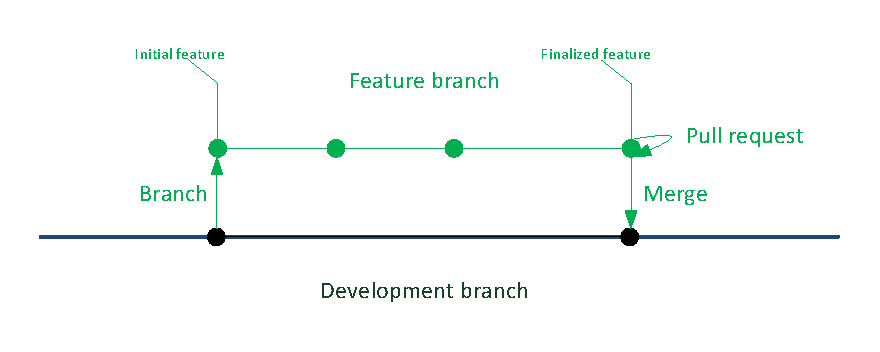
\includegraphics[keepaspectratio,width=\textwidth]{./images/branching.pdf}
\caption{Branching strategie van Canvas.hs}
\label{fig:branching}
\end{center}
\end{figure}

Door deze manier van werken is altijd de development branch goed getest en is het altijd mogelijk om een nieuwe release uit te brengen met de op dat moment volledig geteste features. Iedere release wordt in de master branch uitgebracht.

\todo{staat die hele branchingstrategie niet in hoofdstuk 2, hier alleen even kort herhalen?}

\section{Cabal}
De buildconfiguratie en testconfiguraties worden in de cabal file bijgehouden. Met het commando cabal test kunnen alle tests van het project uitgevoerd worden. Op de website van Canvas.hs staan uitgebreide instructies over het uitvoeren van tests.

\section{Continuous Integration}
Iedere ontwikkelaar zal gedurende de ontwikkeling zijn\todo{anders formuleren geen Engelse woorden er in dumpen} aanpassingen pushen naar de Github repository. De Github repository is gekoppeld met Travis een cloud based continuous integration server. Tests worden automatisch uitgevoerd door Travis na het pushen van iedere commit. Indien een build faalt, zal hierover een bericht in Hipchat geplaatst worden. Doordat builds automatisch getest worden is altijd duidelijk: Welke ontwikkelaar fouten in Canvas.hs introduceert, wat de status van iedere branch is en of een branch gemerged kan worden naar de development branch.

\todo{Beter alle losse delen geschrijven}
\todo{Duidelijkere TODOs schrijven want deze is mij compleet onduidelijk??}
\section{JavaScript} 
Aan de client side wordt gewerkt met JavaScript, het Jasmine test framework wordt gebruikt om de tests te ontwikkelen. Door middel van PhantomJS kunnen de tests vanaf de command line worden uitgevoerd zonder browser. Hierdoor kunnen de tests ook op de build server uitgevoerd worden. Verder zal er gebruik gemaakt worden van de imagediff library om de daadwerkelijk getekende output te testen. Voor het meten van code coverage in JavaScript wordt gebruik gemaakt van Blanket.js.

\section{Haskell}
De Haskellcode in Canvas.hs wordt getest met behulp van ``Hspec''. Hier is voor gekozen omdat Hspec relatief eenvoudig werkt en goed integreert met Cabal. Hierbij kan Hspec automatisch de verschillende tests in een map ontdekken en uitvoeren.

In samenwerking met Hspec wordt QuickCheck gebruikt. Dit veel gebruikte testframework maakt het mogelijk om een groot aantal willekeurige testcases uit te voeren. Dit geeft extra zekerheid over de geteste code aangezien er naast de bekende edge cases, waarvoor tests in Hspec zijn geschreven, ook een groot aantal willekeurige cases wordt getest.